% DO NOT COMPILE THIS FILE DIRECTLY!
% This is included by the other .tex files.

\begin{frame}[t,plain]
\titlepage
\end{frame}

\begin{frame}
\frametitle{A Common Integration}
        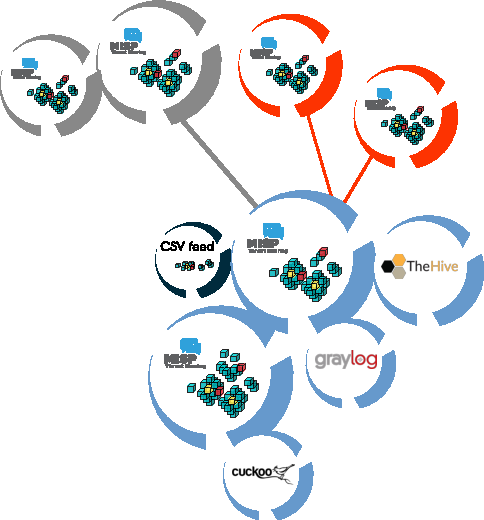
\includegraphics[scale=0.8]{misp-integration-overview.pdf}
\end{frame}

\begin{frame}
\frametitle{Recommended MISP Setup}
    \begin{itemize}
            \item Provisioning your MISP infrastructure depends heavily on the {\bf number of attributes/events} (whether your dataset is below or above ~50 million attributes).
            \item Number of MISP instances and the overall design depends on the following factors:
                    \begin{itemize}
                            \item Is your community private? Are you gathering MISP events from other communities? Are you {\bf publishing events to external} (trusted/untrusted) communities.
                            \item Do you plan to have {\bf automatic tools} (e.g. sandbox analysis or low-value information needing correlation or an analyst workbench) feeding MISP?
                    \end{itemize}
    \end{itemize}
\end{frame}

\begin{frame}
\frametitle{Vendors and Formats}
\begin{itemize}
        \item There is {\bf a jungle of formats} with some vendors having little to no interest in keeping their users autonomous.
        \item Attacks and threats require a {\bf dynamic format} to be efficiently shared (e.g. from financial indicators to personal information).
        \item {\bf Review your current list of formats/vendors} to ensure a limited loss of information, especially when exporting from MISP to other formats (e.g. STIX not supporting financial indicators or taxonomies/galaxies).
\end{itemize}
\end{frame}

\begin{frame}
\frametitle{Use case: Normalizing OSINT and Private Feeds}
\begin{itemize}
        \item Normalizing external input and feed into MISP (e.g. feed importer).
        \item Comparing feeds before import (how many similarities? false-positives?).
        \item Evaluating quality of information before import (warning-list lookup at feed evaluation).
\end{itemize}
\end{frame}


\begin{frame}
\frametitle{Connecting Devices and Tools to MISP}
\begin{itemize}
        \item One of the main goals of MISP is to feed protective or detection tools with data
        \begin{itemize}
            \item IDSes / IPSes (e.g. Suricata, Bro, Snort format as included in Cisco products)
            \item SIEMs (e.g. CEF, CSV or real-time ZMQ pub-sub or Sigma)
            \item Host scanners (e.g. OpenIOC, STIX, yara rule-set, CSV)
            \item Various analysis tools (e.g. Maltego)
            \item DNS policies (e.g. RPZ)
        \end{itemize}
        \item Various ways of exporting this data (downloads of the selected data, full exports, APIs)
        \item The idea was to leave the selection process of the subset of data to be pushed to these up to the user using APIs.
\end{itemize}
\end{frame}


\begin{frame}
\frametitle{SIEM and MISP Integration}
\begin{itemize}
        \item SIEMs and MISP can be integrated with different techniques depending on the processes at your SOC or IR:
        \begin{itemize}
                \item Pulling events (via the API) or indicator lists at {\bf regular intervals} in a given time frame to perform lookups.
                \item Subscribing to the MISP ZMQ {\bf pub-sub channel} to directly get the published events and use these in a lookup process.
                \item {\bf Lookup expansion module} in MISP towards the SIEM to have a direct view of the attributes matched against the SIEM.
        \end{itemize}
        \item The above options can be combined, depending on your organisation or requirements to increase coverage and detection.
\end{itemize}
\end{frame}

\begin{frame}
\frametitle{ZMQ integration: misp-dashboard}
        \begin{itemize}
        \item A dashboard showing live data and statistics from the ZMQ pub-sub of one or more MISP instances.
        \item Building {\bf low-latency software} by consuming pub-sub channel provides significant advantages over standard API use.
        \item Process information in {\bf real-time} when it's updated, created, published or gathered in MISP.
        \item Demo!
        \end{itemize}

\end{frame}

\begin{frame}
    \frametitle{New integrations: IR and threat hunting using MISP}
    \begin{itemize}
        \item Close co-operation with {\bf the Hive project} for IR
        \begin{itemize}
            \item Interact with MISP directly from the Hive
            \item Use both the MISP modules and the {\bf Cortex} analysers in MISP or the Hive directly
        \end{itemize}
        \item Using MISP to support your threat hunting via {\bf McAfee OpenDXL}
        \item (\url{https://securingtomorrow.mcafee.com/business/optimize-operations/expanding-automated-threat-hunting-response-open-dxl})
    \end{itemize}
\end{frame}

\begin{frame}
    \frametitle{The Hive integration}
    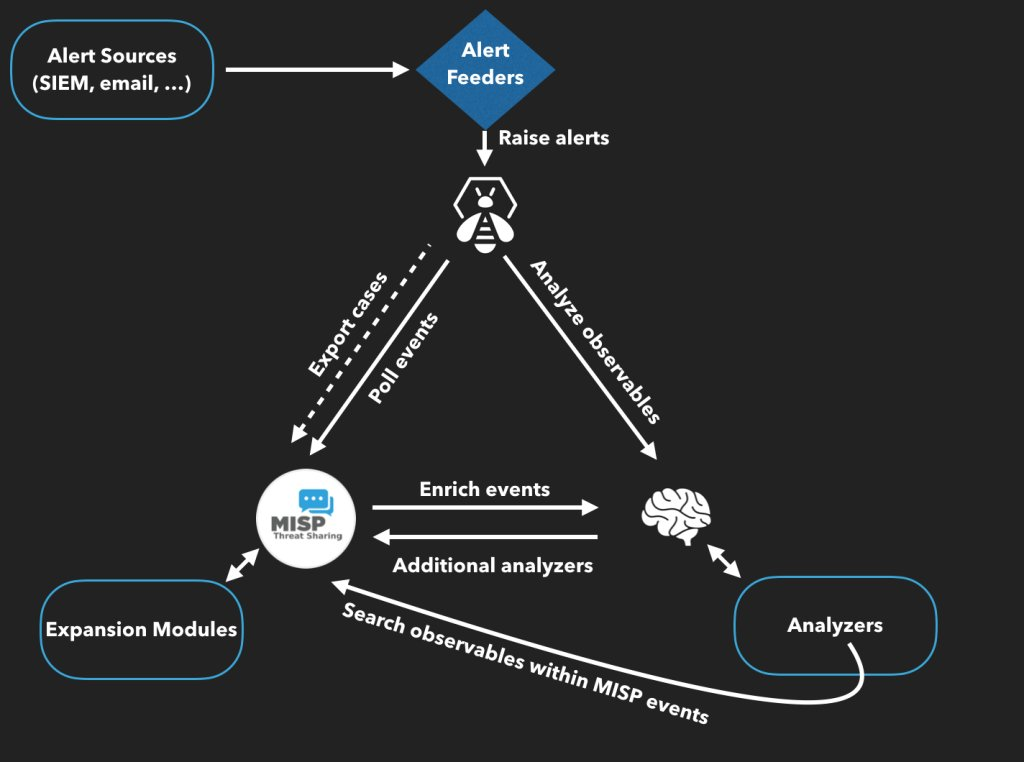
\includegraphics[scale=0.25]{screenshots/cortex.jpg}
\end{frame}

\begin{frame}
\frametitle{Reporting Back from your Devices, Tools or Processes}
As {\bf Sightings} can be positive, negative or even based on expiration, different use cases are possible:
\begin{itemize}
\item {\bf Sightings} allow users to notify a MISP instance about the activities related to an indicator.
\item Activities can be from a SIEM (e.g. Splunk lookup validation or {\bf false-positive feedback}), a NIDS or honeypot devices\footnote{\url{https://www.github.com/MISP/misp-sighting-tools}}.
\item Sighting can affect the API to limit the NIDS exports and improve the NIDS rule-set directly.
\end{itemize}
\end{frame}

\begin{frame}
        \frametitle{Q\&A}
        \begin{itemize}
                \item info@circl.lu (if you want to join the CIRCL MISP sharing community)
                \item \url{https://github.com/MISP/} - \url{http://www.misp-project.org/}
                \item We welcome any contributions to the project, be it pull requests, ideas, github issues,...
        \end{itemize}
\end{frame}

